
\documentclass[aspectratio=169]{beamer}
\usetheme{PaloAlto}
\usepackage[sort]{natbib}
\usepackage[utf8]{inputenc}

% Components of the title page
\logo{
\includegraphics[height=0.4in]{logo.png}}



\title[Métodos Ordinais]{Métodos Ordinais}
\subtitle{Métodos \textit{Borda, Condorcet e Copeland} utilizando python}
\setbeamercovered{transparent}

\beamertemplatenavigationsymbolsempty

\begin{document}



\author[M. Alexandre P. C. Junior]{
    \begin{tabular}{c} 
        \Large
        Alexandre Castro\\
        \footnotesize \href{mailto:im.alexandre07@gmail.com}{im.alexandre07@gmail.com}
    \end{tabular}}

\institute{
    
\includegraphics[height=0.4in]{ime.png}}

\date{06 de outubro de 2020}

\AtBeginSection[]{
    \begin{frame}
        \frametitle{Roteiro}
        \tableofcontents[currentsection]
    \end{frame}
}

\begin{frame}\maketitle\end{frame}


\begin{frame}
    \frametitle{Roteiro}
    \tableofcontents[pausesections]
\end{frame}

\section{Apresentação}
\begin{frame}
    \frametitle{Apresentação}
    Formação Acadêmica
    \begin{itemize}
        \item Graduação em Ciências navais pela Escola Naval (Habilitação em Administração)
        \item Curso de Aperfeiçoamento em Intendência para Oficiais (Centro de Instrução Almirante Newton Braga)
        \item Cursando Pós Graduação em Ciência de Dados na Pontifícia Universidade Católica (PUC-Rio)
    \end{itemize}

\end{frame}

\section{Objetivos da apresentação}
\begin{frame}{Objetivos da apresentação}
    Os principais objetivos da apresentação são:
    \begin{itemize}[<+- | uncover@+>]
        \item Entender os métodos ordinais;
        \item Verificar seu emprego prático; 
        \item \alert{Implementação utilizando linguagem python}
        \item \alert{PROA Software}
    \end{itemize}
\end{frame}

\section{Os Métodos Multicritério}
\subsection{Conceitos}
\begin{frame}{O que são Métodos Multicritério?}
    Os Métodos \textbf{A}poio \textbf{M}ulticritério de à \textbf{D}ecisão(AMD) são ferramentas que auxiliam o decisor/gestor na resolução problemas de decisão em que hajam diferentes objetivos a se considerar, mesmo que, por vezes, sejam de natureza contraditória, como o problema de reduzir custos e aumentar a qualidade. \cite{Almeida2011}
\end{frame}


\begin{frame}{O que são Métodos Multicritério?}
    \begin{block}{}
        Dados Ordinais x Dados Cardinais
    \end{block}
\end{frame}


\subsection{Vantagens dos Métodos Ordinais}
\begin{frame}{Vantagens dos Métodos Ordinais}
    \begin{itemize}
\item Podem ser aplicados com variáveis qualitativas ou quantitativas;
\item Funcionam melhor com variáveis qualitativas(ordinais) e com problemas multicritério;
\item Não necessitam de grande conhecimento em matemática, maior explicapilidade;
\item Zen do python: “Simple is better than complex”;
\item Muitas vezes, o especialista não poderá quantificar os atributos das alternativas;
\item Os atributos são os valores dos critérios para cada alternativa.
    \end{itemize}
\end{frame}

\subsection{O Método de Borda}
\begin{frame}{O Método de Borda}
    O método de Borda é considerado um método de avaliação multicritério e busca avaliar as alternativas que melhor se ajustem aos critérios definidos. \cite{Barros2020}
\end{frame}

\begin{frame}{O Método de Borda}
\framesubtitle{O algorítimo}
   \begin{enumerate}
       \item Selecionar as alternativas e critérios do problema;
       \item Avaliar as alternativas em relação a cada critério (definindo seus atributos);
       \item Ordenar as alternativas de acordo com cada critério;
       \item atribuir pontos de acordo suas classificações em cada critério (a melhor recebe 1, a segunda, 2 e assim sucessivamente);
       \item Somar os pontos de cada alternativa; e
       \item Ordenar as alternativas de maneira crescente conforme o somatório de pontos (a que tiver menos pontos, será a melhor).
   \end{enumerate}
\end{frame}

\begin{frame}{O Método de Borda}
\framesubtitle{O algorítimo}
\begin{table}[]
    \centering
\begin{tabular}{|l|r|r|r|}
\hline
{} &  criterio1 &  criterio2 &  criterio3 \\
\hline
alternativas &            &            &            \\
\hline
alternativa1 &        100 &        229 &        330 \\
\hline
alternativa2 &       2231 &          3 &         12 \\
\hline
alternativa3 &       3300 &      11124 &       2341 \\
\hline
\end{tabular}
    \caption{Dados de entrada do problema}
    \label{tab:borda_entrada}
\end{table}

\only<2>{\begin{table}[]
    \centering
\begin{tabular}{|l|r|r|r|}
\hline
{} &  criterio1 &  criterio2 &  criterio3 \\
\hline
alternativa3 &                1 &                1 &                1 \\
\hline
alternativa2 &                2 &                3 &                3 \\
\hline
alternativa1 &                3 &                2 &                2 \\
\hline
\end{tabular}
    \caption{Tabela com dados ordenados}
    \label{tab:borda_ordenado}
\end{table}
}

\only<3>{\begin{table}[]
    \centering
    
\begin{tabular}{|l|r|r|r|r|}
\hline
{} &  criterio1 &  criterio2 &  criterio3 &  soma \\
\hline
alternativa3 &                1 &                1 &                1 &     3 \\
\hline
alternativa1 &                3 &                2 &                2 &     7 \\
\hline
alternativa2 &                2 &                3 &                3 &     8 \\
\hline
\end{tabular}
    \caption{Tabela com dados ordenados}
    \label{tab:borda_decisao}
\end{table}
}
\end{frame}



\subsection{O Método de Condorcet}
\begin{frame}{O Método de Condorcet}
\framesubtitle{Definição}
Segundo \cite{Netto2003}, o método de Condorcet trabalha com relações de superação entre as alternativas, sendo o precursor da atual escola francesa de multicritério. A partir das relações de superação entre as alternativas, é possível construir um grafo direcionado, permitindo uma análise visual do problema.

As alternativas são comparadas sempre duas a duas e constrói-se um grafo  que expressa a relação entre
elas.
\end{frame}

\begin{frame}{O Método de Condorcet}
\framesubtitle{O algorítimo}
   \begin{itemize}
       \only<1>{\item Selecionar as alternativas e critérios do problema;
       \item Avaliar as alternativas em relação a cada critério (definindo seus atributos);
       \item Comparar as alternativas aos pares e dentro de cada critério;
       \begin{itemize}
           \item Construir 2-tuplas de alternativas sem reposição (análise combinatória);
           \item Fazer o produto cartesiano entre o conjunto de tuplas e o conjunto de critérios; e
           \item Atribuir os valores (-1, 0 e 1) de acordo com a relação de superação.
       \end{itemize}}
       \only<2>{
       \item Montar as matrizes de comparação intracriterial;
       \item Soma das matrizes geradas para cada critério;
       \item Aplicação da seguinte função:
       \begin{equation}
           F(x) = \begin{cases}
           +1 & \text{Se}~ \sum \geq +1 \\
           0 & \text{Se}~ \sum = 0 \\
           -1 & \text{Se}~ \sum \leq -1 \\
           \end{cases}
       \end{equation}}
    \end{itemize}
\end{frame}

\begin{frame}{O Método de Condorcet}
    \framesubtitle{Exemplo}
    \only<1>{
    \begin{table}[]
        \centering
\begin{tabular}{|l|r|r|r|}
\hline
{} &  infraestrutura &  servicos &  acessibilidade \\
\hline
alternativas &                 &           &                 \\
\hline
alternativa1 &               1 &         4 &               3 \\
\hline
alternativa2 &               4 &         1 &               5 \\
\hline
alternativa3 &               5 &         5 &               4 \\
\hline
alternativa4 &               3 &         5 &               2 \\
\hline
\end{tabular}

        \caption{Dados sobre 4 cidades utilizando a escala likert}
        \label{tab:condorcet_entrada}
    \end{table}}
    
\end{frame}

\begin{frame}{O Método Condorcet}
\framesubtitle{Exemplo}
\only<1>{
\begin{block}{}
\centering
infraestrutura
\end{block}
    \begin{table}[]
\begin{tabular}{|l|r|r|r|r|}
            \hline
            {} &  alternativa1 &  alternativa2 &  alternativa3 &  alternativa4 \\
            \hline
            alternativa1 &             0 &            -1 &            -1 &            -1 \\
            \hline
            alternativa2 &             0 &             0 &            -1 &             1 \\
            \hline
            alternativa3 &             0 &             0 &             0 &             1 \\
            \hline
            alternativa4 &             0 &             0 &             0 &             0 \\
            \hline
        \end{tabular}
        \caption{Dados sobre infraestrutura}
        \label{tab:condorcet_infraestrutura}
    \end{table}
    }
\only<2>{
\begin{block}{}
\centering
servicos
\end{block}

    \begin{table}[]
        \centering
\begin{tabular}{|l|r|r|r|r|}
    \hline
    {} &  alternativa1 &  alternativa2 &  alternativa3 &  alternativa4 \\
    \hline
    alternativa1 &             0 &             1 &            -1 &            -1 \\
    \hline
    alternativa2 &             0 &             0 &            -1 &            -1 \\
    \hline
    alternativa3 &             0 &             0 &             0 &             0 \\
    \hline
    alternativa4 &             0 &             0 &             0 &             0 \\
    \hline
\end{tabular}
        \caption{Dados sobre servicos}
        \label{tab:condorcet_servicos}
    \end{table}
}
\only<3>{
\begin{block}{}
\centering
    acessibilidade
\end{block}

    \begin{table}[]
        \centering
    \begin{tabular}{|l|r|r|r|r|}
        \hline
        {} &  alternativa1 &  alternativa2 &  alternativa3 &  alternativa4 \\
        \hline
        alternativa1 &             0 &            -1 &            -1 &             1 \\
        \hline
        alternativa2 &             0 &             0 &             1 &             1 \\
        \hline
        alternativa3 &             0 &             0 &             0 &             1 \\
        \hline
        alternativa4 &             0 &             0 &             0 &             0 \\
        \hline
    \end{tabular}
        \caption{Dados sobre acessibilidade}
        \label{tab:condorcet_acessibilidade}
    \end{table}
}

\only<4>{
\begin{block}{}
\centering
    Somatório das Matrizes
\end{block}

    \begin{table}[]
        \centering
    \begin{tabular}{|l|r|r|r|r|}
\hline
{} &  alternativa1 &  alternativa2 &  alternativa3 &  alternativa4 \\
\hline
alternativa1 &             0 &            -1 &            -3 &            -1 \\
\hline
alternativa2 &             0 &             0 &            -1 &             1 \\
\hline
alternativa3 &             0 &             0 &             0 &             2 \\
\hline
alternativa4 &             0 &             0 &             0 &             0 \\
\hline

\end{tabular}
        \caption{Somatório das Matrizes}
        \label{tab:matriz_decisao}
    \end{table}
}

\only<5>{
\begin{block}{}
\centering
    Matriz de Decisão
\end{block}

    \begin{table}[]
        \centering
\begin{tabular}{|l|r|r|r|r|}
    \hline
{} &  alternativa1 &  alternativa2 &  alternativa3 &  alternativa4 \\
    \hline
alternativa1 &             0 &            -1 &            -1 &            -1 \\
    \hline
alternativa2 &             0 &             0 &            -1 &             1 \\
    \hline
alternativa3 &             0 &             0 &             0 &             1 \\
    \hline
alternativa4 &             0 &             0 &             0 &             0 \\
    \hline
\end{tabular}
        \caption{Matriz de Decisão}
        \label{tab:matriz_decisao}
    \end{table}
}
\end{frame}

\begin{frame}{O Método Condorcet}
    \framesubtitle{Grafo}
    \centering
    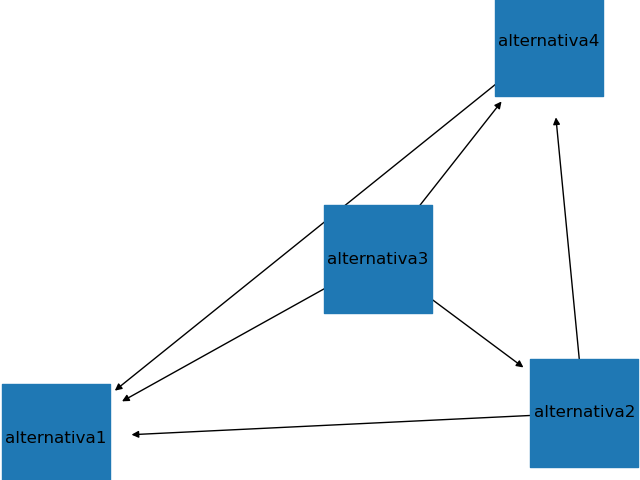
\includegraphics[height=2in]{grafo_condorcet.png}
\end{frame}

\begin{frame}{O Método Condorcet}
    \framesubtitle{Observação}
    \begin{block}{Ciclo de intransitividade}
    E se as alternativas obtiverem o mesmo número de vantagens em relação às demais?
    \end{block}
    O ciclo de intransitividade é a intransitividade da escolha coletiva, mesmo que essa escolha seja baseada em escolhas transitivas. Ou seja, mesmo que, de par em par, seja possível encontrar uma alternativa superior, no geral, será impossível chegar a um resultado.
    Exemplo: Tendo três alternativas, sendo \textbf{A, B e C}. Podemos chegar à conclusão de que \textbf{A domina B}, \textbf{B domina C} e \textbf{C domina A}. A esse ciclo de relações de superação, dá-se o nome de \textbf{paradoxo de Condorcet}.\cite{Pereira2008}
\end{frame}



\begin{frame}{O Método de Copeland}
\framesubtitle{Conceito}
O método de Copeland é baseado no de Condorcet, possuindo a vantagem de sempre gerar uma ordenação total, evitando o problema do ciclo de intransitividade. \cite{Gomes2011}

\end{frame}

\subsection{O Método de Copeland}
\begin{frame}{O Método de Copeland}
\framesubtitle{O algorítimo}
Em relação à execução do método, serão realizados os mesmos passos do método de Condorcet, porém, serão consideradas as relações opostas (compara A com B e B com A).
Logo, temos o seguinte algorítimo:
\begin{itemize}
    \item Realizar o método de Condorcet;
    \item Como as alternativas serão comparadas em "dois turnos", basta obter a matriz transposta da matriz de decisão gerada pelo método anterior com os sinais trocados;
    \item Somar a nova matriz com a matriz obtida com o método de Condorcet;
    \item Somar as relações de superação por linha (ou alternativa);
    \item Ordenar as alternativas de acordo com o somatório alcançado.
\end{itemize}

\end{frame}

\begin{frame}{Método de Copeland}
\framesubtitle{Exemplo}
    
\only<1>{
\begin{block}{}
\centering
    Matriz de Decisão (Copeland)
\end{block}

    \begin{table}[]
        \centering
\begin{tabular}{|l|r|r|r|r|}
    \hline
{} &  alternativa1 &  alternativa2 &  alternativa3 &  alternativa4 \\
    \hline
alternativa1 &             0 &            -1 &            -1 &            -1 \\
    \hline
alternativa2 &             0 &             0 &            -1 &             1 \\
    \hline
alternativa3 &             0 &             0 &             0 &             1 \\
    \hline
alternativa4 &             0 &             0 &             0 &             0 \\
    \hline
\end{tabular}
        \caption{Matriz de Decisão Gerada pelo método de Condorcet}
        \label{tab:matriz_decisao_condorcet}
    \end{table}
}
\only<2>{
\begin{block}{}
\centering
    Matriz transposta com sinal trocado
\end{block}

    \begin{table}[]
        \centering
\begin{tabular}{|l|r|r|r|r|}
    \hline
{} &  alternativa1 &  alternativa2 &  alternativa3 &  alternativa4 \\
    \hline
alternativa1 &             0 &             0 &             0 &             0 \\
    \hline
alternativa2 &             1 &             0 &             0 &             0 \\
    \hline
alternativa3 &             1 &             1 &             0 &             0 \\
    \hline
alternativa4 &             1 &            -1 &            -1 &             0 \\
    \hline
    \end{tabular}
        \caption{Matriz com as comparações inversas}
        \label{tab:condorcet_transposta}

    \end{table}
}

\only<3>{

\begin{block}{}
\centering
    Matriz com as comparações em "dois turnos"
\end{block}
 \begin{table}[]
        \centering
\begin{tabular}{|l|r|r|r|r|}
    \hline
{} &  alternativa1 &  alternativa2 &  alternativa3 &  alternativa4 \\
    \hline
alternativa1 &             0 &            -1 &            -1 &            -1 \\
    \hline
alternativa2 &             1 &             0 &            -1 &             1 \\
    \hline
alternativa3 &             1 &             1 &             0 &             1 \\
    \hline
alternativa4 &             1 &            -1 &            -1 &             0 \\
    \hline
\end{tabular}
        \caption{Soma das matrizes anteriores}
        \label{tab:matriz_final_copeland}
    \end{table}
}

\only<4>{

\begin{block}{}
\centering
    Matriz de Decisão
\end{block}
 \begin{table}[]
        \centering
\begin{tabular}{|l|r|r|r|r|r|}
    \hline
{} &  alternativa1 &  alternativa2 &  alternativa3 &  alternativa4 &  soma \\
    \hline
alternativa3 &             1 &             1 &             0 &             1 &     3 \\
    \hline
alternativa2 &             1 &             0 &            -1 &             1 &     1 \\
    \hline
alternativa4 &             1 &            -1 &            -1 &             0 &    -1 \\
    \hline
alternativa1 &             0 &            -1 &            -1 &            -1 &    -3 \\
    \hline
\end{tabular}
        \caption{Matriz de decisão}
        \label{tab:matriz_decisao_copeland}
    \end{table}

}
\end{frame}

\section{Prática com linguagem Python}
\begin{frame}{Prática com linguagem Python}
    \centering
    
\includegraphics[height=2.8in]{talkischeap.jpg}
\end{frame}

\begin{frame}
    \frametitle{Conclusão}
    \centering
        OBRIGADO!\\
        \begin{block}{}
            Contatos:
        \end{block}


    \begin{tabular}{cc}
        Linkedin: & \href{https://www.linkedin.com/in/alexandre-castro-45593415a/}{
\includegraphics[height=0.3in]{linkedin.png}}\\
        \hline
        Github:  & \href{https://www.github.com/im-alexandre}{
\includegraphics[height=0.3in]{github.png}}\\
        \hline
        E-mail:  &  \href{mailto:im.alexandre07@gmail.com}{
\includegraphics[height=0.3in]{gmail.png}}\\
        \hline
        Repositório da aula:  &  \href{https://github.com/im-alexandre/aula_metodos_ordinais}{
\includegraphics[height=0.3in]{github.png}/aula\_metodos\_ordinais}\\
        \hline
    \end{tabular}
\end{frame}

\begin{frame}{Referências}
\bibliographystyle{apalike}
\bibliography{Bibliografia.bib}
\end{frame}

\end{document}
